\section{Durchführung}
\label{sec:Durchführung}

Zur Bestimmung der Trägheitsmomente der verschiedenen Körper müssen zunächst die
Apparaturkonstanten, also die Winkelrichtgröße $\symbf{D}$ und das Trägheitsmoment
der Drillachse $I_\mathrm{D}$, bestimmt werden.
\begin{figure}
  \centering
  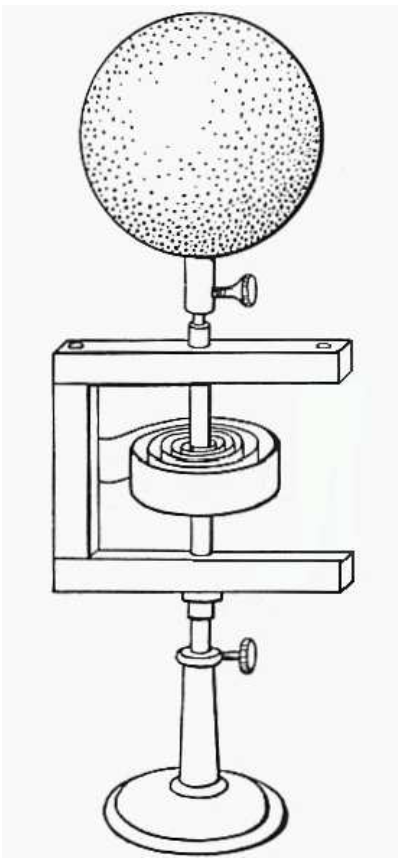
\includegraphics[width=100pt]{Aufbau.png}
  \caption{Aufbau der Apparatur, hier mit eingespannter Kugel \cite{Versuchsanleitung}}
  \label{fig:Aufbau}
\end{figure}


Zur Bestimmung der Winkelrichtgröße wird ein Stab in die Apparatur eingeschraubt und
um verschiedene Winkel $\phi$ ausgelenkt. Mit einer Federwaage wird die im Abstand
$\symbf{r}$ wirkende rücktreibende Kraft gemessen. Dabei muss darauf geachtet werden,
dass der Auslenkungswinkel nicht größer als 360° ist, um inelastische Verformungen der
Spiralfeder zu vermeiden, und darauf, dass die Kraft immer in Richtung des Einheitsvektors
$\symbf{e}_\mathrm{{\phi}}$ gemessen wird, da ansonsten der Zusammenhang aus \eqref{eqn:winkelrg}
nicht mehr gilt. Die Messung wird für zehn verschiedene Winkel $\phi$ durchgeführt.

Zur Bestimmung des Trägheitsmomentes der Drillachse werden an den zuvor eingespannten
Stab zwei gleich große Massen im jeweils gleichen Abstand $\symbf{r}$ von der
Drehachse gehängt. Danach wird die Stange aus ihrer Ruhelage um einen kleinen Winkel
$\symbf{\phi}$ ausgelenkt und die Schwingungsdauer bestimmt. Dabei wird bereits bei
der Messung über zwei Periodendauern gemittelt. Die Messung wird für zehn verschiedene
Abstände $\symbf{r}$ der Massen von der Drehachse durchgeführt. Zum Schluss werden
noch die Massen der beiden Gewichte bestimmt.

Im Anschluss daran sollen die Trägheitsmomente zweier Körper, hier das einer Kugel und
das eines Zylinders, bestimmt werden. Dafür wird zunächst der jeweilige Körper in
die Apparatur eingespannt und anschließend die Schwingungsdauer bei einer Auslenkung
zwischen etwas 60° und 100° gemessen. Bei der Messung wird hier bereits über drei
Periodendauern gemittelt. Je nach verteilung der Messwerte wird die Messung mehr
oder weniger oft wiederholt. Bei kleinen Abweichungengenügen bereits wenige Messungen,
bei größeren Abweichungen werden entsprechend mehr benötigt. Am Ende müssen noch die
geometrischen Abmessungen der Körper mithilfe einer Schieblehre, sowie die Massen der
Körper bestimmt werden.

Für die Puppe soll das Trägheitsmoment in zwei verschiedenen Körperhaltungen bestimmt
werden. Als erste Körperhaltung wurden angelegte Arme und nach vorne und hinten
abgespreizte Beine gewählt. Die Puppe wird in die Apparatur eingespannt und erneut
wird die Periodendauer bei einer Auslenkung zwischen 60° und 100° über drei
Periodendauern gemittelt gemessen. Auch hier wird die Messung je nach Bedarf
unterschiedlich häufig wiederholt. Daraufhin wird die Puppe in eine andere
Körperhaltung gebracht. Hier wurden nach vorne und hinten abgespreizte Beine,
sowie zu den Seiten ausgestreckte Arme gewählt. Bei der Messung wird genau so
verfahren wie bei der anderen Körperhaltung.
